\documentclass[a4paper,12pt]{article}
\usepackage[utf8]{inputenc}
\usepackage{mathtools}

% Allow the change of line spacing
\usepackage{setspace}
\usepackage{tabularx}
\usepackage{graphicx}
\usepackage[usenames,dvipsnames,table]{xcolor}

%\usepackage{hyperref}
%\usepackage{breakurl}

%opening
%\title{Trainmining}
%\author{Grupo de Sistemas Inteligentes \\ Universidad Politécnica de Madrid}


\begin{document}
\newcommand\litem[1]{\item{\bfseries #1 }}
\renewcommand{\arraystretch}{1.5} %Makes tables less crammed

\newcommand\headcell[1]{%
  \multicolumn{1}{c|}{\cellcolor{MidnightBlue}\bfseries\sffamily\textcolor{white}{#1}}
}

%\renewcommand{\abstractname}{Executive Summary}
%\begin{abstract}
%
%\end{abstract}

% Set line spacing to 1.5
\onehalfspacing

% Begin a new titlepage. Tit	lepages have special settings like the absence of page numbers.
\begin{titlepage}
\sffamily
% Set the text of the page to right-aligned until \end{flushright}
\begin{flushright}

% Set the space between right page border and text to 2.5cm
\rightskip=-1cm

% Show an image at this position

\includegraphics[scale=1]{./img/logoGSI.png} 
%\includegraphics[bb=0 0 204 110]{web40logo.png}

% Skip a little space
\bigskip
\bigskip
\bigskip



% Create a title for the document and write it in bold font
\LARGE{\textbf{Deliverable 3. Knowledge Discovery results.}}
% Again, do a line break
\linebreak
% Create a subtitle
\large{Evaluation and interpretation.}

% Skip some space
%\bigskip
%\bigskip
%\bigskip
%\bigskip
\bigskip

% Write in very large letters
\LARGE{Grupo de Sistemas Inteligentes}
\linebreak
\large{Departamento de Ingeniería de Sistemas Telemáticos}
% Do a line break right after the \LARGE{...} text
\linebreak
% Write in large letters
\large{Universidad Politécnica de Madrid.}

% Skip some space
\bigskip
\bigskip
\bigskip
\bigskip
\bigskip
\bigskip

\large{Project Report}

% Skip some space
\bigskip

\normalsize{Madrid, October 2012}

% Skip some space
\bigskip
\bigskip
\bigskip
\bigskip
\bigskip
\bigskip
\bigskip
\bigskip
\bigskip
\bigskip
\bigskip
\bigskip
\bigskip
\bigskip
\bigskip
\bigskip

% Provide some author information
\normalsize{Authors:}
\linebreak
\large{Adrián Pérez Orozco}
\linebreak
\large{Álvaro Carrera Barroso}
\linebreak
\large{Carlos A. Iglesias Fernández}

% End right-alignment at this point
\end{flushright}
% End the title page
\end{titlepage}

%\maketitle

\pagenumbering{roman}
\section*{Executive Summary}
\addcontentsline{toc}{section}{Executive Summary} % si queremos que aparezca en el índice

This document describes the main knowledge discovery procedure performed for the \emph{Trainmining} project. After the already described and finished steps of goal definitions, data analysis and preprocessing, this step focuses on the data mining procedures themselves: the actual extraction of the knowledge from the available databases.

All the existing data mining algorithms have been analised and classified in order to find the most appropriate for our purposes. After this survey, two main options were found to be the best potential methods to approach our problem: association rules based on frequent patterns and bayesian networks.

The first method consists on finding frequent patterns in our databases in order to be used as predictive rules. Different algorithms already exist to mine these frequent patterns, of which we will select the most advanced and efficient one: cSPADE. In order to build useful prediction rules, two factors have to be taken into account: temporal adequation (patterns that do not run for too long or inadequate periods) and their actual precision (removing the \emph{noise} introduced by events which are frequent but do not offer good predictive information).

In order to being able to adequately extrapolate our acquired knowledge to periods not covered by our historical data, we must try and remove the specific characteristics of these databases. For this purpose, a special validation method will be used: the \emph{k-fold cross validation method}. This method separates the database into \emph{k} different learning and result sets and iterates the whole learning/validation procedure in all of them. This way, the result is a system with an average performance for all the different parts of the database, which avoids overfitting of our predictive rules for any specific dataset.

The second method uses a mathematic tool: bayesian networks. These networks are graphs representing all the possible events in our system as different nodes. These nodes have two possible states, indicating whether the alarm has happened during the current period or not; as well as an associated probability for each of the states. These probabilities are conditioned to the probability of the rest of states in the network, so that when a probability changes (i.e. we have certainty of an event having happened) the probabilities of the rest of the network are affected as well to reflect the new system status.

Using these models we can know the probability of a determinate event happening after the events already known of the current observation period. This allows us to predict events in a similar fashion than with our rule-based model, although computation of probabilities is completely different. In this direction, the same evaluation and validation approach will be followed: using \emph{k-fold cross validation} and treating the probability given for each graph node as if it was a rule-based prediction.

After evaluating both models, our rule-based approach is seen to perform much better than bayesian networks. Therefore, additional tuning and development will be performed in order to improve our rule-based model, while the bayesian model development will be put on hiatus due to the high amount of work which would be required just to achieve the same performance level.

Finally, an analysis of the results is gathered in this document, which allows us to see at first glance the kind of results obtained and their performance rating.

\newpage
\tableofcontents % indice de contenidos
\addcontentsline{toc}{section}{Contents} % para que aparezca en el indice de 
\cleardoublepage
\addcontentsline{toc}{section}{List of Figures} % para que aparezca en el indice de contenidos
\listoffigures % indice de figuras

\cleardoublepage
\addcontentsline{toc}{section}{List of tables} % para que aparezca en el indice de contenidos
\listoftables % indice de tablas
\cleardoublepage

\setcounter{page}{1}
\pagenumbering{arabic}
\section{Introduction}
In previous stages of our project we have performed preliminary analysis on our data (mostly statistical) as well as the necessary preprocessing to apply different learning techniques in the following stages. Once we have completed these tasks, it is now time to perform the techniques from which the actual knowledge will be obtained.

This step, usually refered to as \emph{Data Mining} is the most important in the whole \emph{knowledge discovery} procedure. Although data analysis and preprocessing do have a big impact on the quality of the results we will be able to achieve in the end, the choice of an appropriate data mining algorithm is essential for the whole procedure to work.

\section{Data mining}\label{sec:datamining}
In order to find the most adequate techniques for knowledge discovery in our project, we will start making a general survey on all the available techniques. Due to the vast amount of already existing implementations available for each of the different data mining categories, we won't have to make an implementation from scratch but adapt one of the already existing implementations to the characteristics of our problem by setting the necessary constraints.

To begin with, we will describe the categories in which all the different algorithms are usually classified. This classification is usually made as follows:

\begin{enumerate}
 \litem{Classification:} Consists on finding functions to map items into already existing classes according to their parameters or characteristics.
 \litem{Regression:} Algorithms aimend to learn functions to predict the value of some variables from other variables or previous values of the same one.
 \litem{Segmentation:} Consists on finding a set of clusters or segments in which the existing items can be categorised.
 \litem{Summarization:} Algorithms used to find compact description for existing data items.
 \litem{Association:} Learning significant relations or dependencies between different variables.\cite{Zhao2003association}.
 \litem{Sequence analysis:} Finding frequent sequences or episodes in data~\cite{zhao2003sequential,weiss2002predicting}.
\end{enumerate}

\emph{Segmentation} and \emph{summarization} algorithms seem to be obviously out of the question, as their functionality differs completely from the objectives we want to achieve in our project. \emph{Regression} algorithms are inadequate as well due to the nature of our data. We do not count on variables whose future value we want to predict.

\emph{Sequence analysis} seems to be the most appropriate category at at first glance: we count on historic data from the past and we want to find event patterns from which we can foresee future events. Patterns which are frequent offer useful information in this direction. If we know a set of several events which often happen in the same sequence, we can expect the later events in the sequence to happen once we have already seen the first ones.

These sequences offer a good starting point, but it is important to realize that \emph{frequency} in a pattern refers to the total of events happening during the observated period, and does not indicate in any way the \emph{probability} of the last events in a sequence to happen once the first ones have been acknowledged. In other words, we want to obtain predictions with a high \emph{probability} rather than a high \emph{frequency}.

In this direction, we will use the approach of the \emph{association} algorithms. Using frequent sequences as an starting point, we will build \emph{association rules} which will relate events in the form of boolean variables.

\emph{Classification} algorithms might not seem like a good choice at first, as we do not have the need to classificate the events into any existing categories. However, if we define an appropriate set of categories and an appropriate model of items to classify, classification algorithms can be actually useful for our tasks. If we model the current events as the \emph{item} to classify, and the possible categories as the possible events which can happen in the future, we can actually classify the current situation (defined by the events which have already happened) into possible categories each defining what would happen next.

At this point we have two appropriate approaches. In first place, we can build association rules based on sequence analysis made in our data. As a second approach, we can follow a classification method. In order to build our rule-based model, we will use \emph{cSPADE}, an algorithm which provides a convenient way to find frequent patterns. Further details on this model and the selected algorithm is given in section~\ref{sec:rule_model}. For our classification model, we will use \emph{bayesian networks} as explained in section~\ref{sec:bayesian}

\section{Model based in association rules}\label{sec:rule_model}
As we mentioned previously, one of our options to approach our problem is the construction of a model based on association rules. This approach consists on building association predictive rules using frequent secuences in our available data as a base.

First of all we must therefore obtain all potential sequential information (patterns) from our database, as mentioned. These sequences will be of the form $\{A, B\} \longrightarrow \{C, D\} \longrightarrow \{E, F\}$ and will serve as a basis to build candidate \emph{association rules}. This step is explained with further details on section~\ref{sec:mining_sequences}.

Using the frequent sequences obtained from the first step, we can build \emph{candidate association rules}. Candidate association rules are of the form $\{A, B\} \xrightarrow{T} \{C\}$. It is important to notice that in these rules we are putting additional temporal information (a distance of T between terms). This temporal information is not implicit in our previous temporal sequences, but can be inferred from the conditions used on the process to obtain them. This will be explained in detail in section~\ref{sec:assoc_rules}.

Finally, we must check which of these \emph{candidate association rules} are actually good predictive rules, and obtain a precise measure of \emph{how good} they are. Specifically, we will measure the \emph{certainty} (precision) of the predictions made by using these rules and the \emph{amount of events} (recall) they are able to predict. This step will be explained in detail in section~\ref{sec:validation_evaluation}.

The whole procedure can be summarized in the following steps:
\begin{enumerate}
\item Mining frequent sequences
\item Building candidate association rules
\item Validate the obtained rules
\end{enumerate}

These steps will be further described in the following sections.

\subsection{Obtaining frequent sequences}\label{sec:mining_sequences}
The first step for our chosen approach is to find frequent sequences in our datasets. Frequent sequences will be good candidates from which we can be able to obtain association rules -- if there is an unknown causal relation between two events, they will appear together considerably often. Several algorithms have been developed in the past in order to approach this task of finding frequent sequences. Some examples are the \emph{GSB} algorithm and the \emph{SPADE} algorithm, being the later an alternative to the first with better performance and results.

The procedure of finding frequent sequences in a dataset mainly consists on an iterative analysis of all the possible combinations of elements of the database in sequences. For example, the GSB algorithm can be roughly described as follows:

\begin{enumerate}
\item All the possible items (events) of the database are counted. These elements can be seen as sequences of length 1, which will be subsequences of any other larger sequence.
\item All the possible length 2 candidates are generated, as combination of length 1 sequences
\item The database is scanned to calculate the support of generated length 2 candidates
\item Length 3 candidates are generated as addition of length 1 sequences to length 2 sequences whose support is higher than a given minimum
\item The process is repeated till no candidates have high enough support
\end{enumerate}

The support of a sequence is calculated as the number of times it happens in our dataset. The support is usually expressed as a percentage of the whole amount of sequences in the database, but it is important to note that this parameter is not related in any way with the confidence or precision of any prediction we might do with the given pattern. A deeper approach on this issue will be described later in this document.

More information on GSB and SPADE algorithms can be found in \cite{zaki2001spade, zhao2003sequential, srikant1996mining}. Although It is not our priority now to study these algorithms in depth, previous work shows a better performance for SPADE than for GSB, and therefore it will be our algorithm of choice for our work. Furthermore, SPADE implementations are conveniently available in R libraries, which will allow us to easily execute the algorithm on our datasets.

\subsubsection{Defining constraints}
One of the main problems we find when we look for frequent sequences in our database, is that not any sequence -- although frequent -- is useful for our purposes. In the end our goal is to make predictions, for which obtaining these frequent patterns is useful. However, our project context -- and sometimes common sense -- may put additional conditions on \emph{which} kind of predictions are useful; and therefore, \emph{which} kind of patterns we must look for.

For instance, due to the characteristics of our systems, it might not be possible to perform maintenance tasks in short periods of time. Sequences showing us that \emph{A} always breaks within one hour after \emph{B} breaking might not be useful even if we can obtain a very high certainty of that prediction. If we need to buy new pieces to fix B, and those pieces are usually delivered in terms of weeks, knowing that \emph{B} will break one hour before it breaks would not give us any advantage over waiting for it to break and notice without any prediction.

In other words: we need to define temporal constraints in order to obtain sensible predictions\cite{zaki2000cspade}. These constraints are the following:

\begin{description}
\item[Observation time.] We must define for how long we want to take events into account. For example, our predictions for tomorrow will be most likely be made taking into account today's events, as those from last week are less likely to be related with those happening in the short future.
\item[Minimum gap.] This is the minimum amount of time in which we want to predict events. For instance, a gap of 0 would result in predictions for events simultaneous to the observed ones, while a gap of 1 would result in predictions only for the following observation periods.
\item[Maximum gap.] The maximum amount of observations between events in our sequences. By fixing it to the same amount as minimum gap we can obtain sequences with a fixed gap between events.
\item[Maximum window.] This is the maximum temporal length for our sequences. It is important to stress that this is the length of the whole sequence, while the gap is the separation of events within a sequence.
\end{description}

Given these constraints, we have sequences with the following structure:

$$\{A, B\} \xrightarrow{T_1} \{C, D\} \xrightarrow{T_2} \{E, F\}$$

Where $mingap \leq \{T_1, T_2\} \leq maxgap$, and $T_1+T_2 \leq maxwin$. It is important to remark that these temporal conditions are not inherent to the sequences obtained by the SPADE algorithm. As we mentioned in section \ref{sec:mining_sequences}, sequences are built from all the possible combination of events, and then their support is calculated by checking how many times that sequence appears in the database. It is in support calculation where these constraints apply, but the candidate sequences do not contain any temporal information at all. We will only know that their values will be comprised within the ranges we have defined.

In this sequence we have three terms with two events each. In order to build association rules, it is very convenient to limit the number of terms to two -- a single \emph{antecedent} and a single \emph{consequent}. Furthermore, it is very convenient to limit the number of events to one, in order to make individual predictions for each of the events (which may have, for example, different certainties). 

Therefore, the previous example sequence can be divided in three subsequences of two terms:
$$\{A, B\} \longrightarrow \{C, D\}$$
$$\{C, D\} \longrightarrow \{E, F\}$$
$$\{A, B\} \longrightarrow \{E, F\}$$

And, furthermore, each of them can be divided into two subsequences with only one item in the last term:

$$\{A, B\} \longrightarrow \{C\}$$
$$\{A, B\} \longrightarrow \{D\}$$
$$\{C, D\} \longrightarrow \{E\}$$
$$\{C, D\} \longrightarrow \{F\}$$
$$\{A, B\} \longrightarrow \{E\}$$
$$\{A, B\} \longrightarrow \{F\}$$

These sequences are in fact subsequences of the original one, and therefore their individual support values will always be higher than the support original one. This means that these subsequences will already have been obtained as frequent sequences by the SPADE algorithm, without the need of performing division on the longer sequences. As a result, we can simply drop the sequences whose length or complexity is inconvenient for our purposes, as their shorter subsequences will be already found by SPADE.

This results in additional length constraints:
\begin{description}
\item[Maximum terms.] The maximum number of terms in the sequence. In our previous example, we should have set it to \emph{2}.
\item[Maximum items per term.] This condition defines the maximum amount of items in each of the terms of the sequence. This is \emph{not exactly} what we wanted to achieve with our second division of sequences, as we only want to apply this condition to the last term and not to all of them. In our previous example, we would have to set this limit to 1 but only for the last term of the sequence.
\end{description}

Both these groups of constraints must be applied within the process of the algorithms which will obtain the frequent sequences from our database. The length constraints will limit the construction of \emph{candidate sequences} and the temporal constraints will put conditions to the calculation of \emph{sequence support}. Its implementation must therefore be made into the sequence mining algorithms.

An extended version of the SPADE algorithm has been developed to include some of these constraints which were not contemplated by the original SPADE implementation. The \emph{cSPADE} algorithm\cite{zaki2000cspade,wu2010sequential} provides an implementation taking into account all these mentioned conditions. It is available as an R implementation under the library \emph{arulessequences}\cite{hahsler2011arules}. The only constraint which we are not directly able to define as a cSPADE condition is the maximum number of items in the last term of the sequence, as the condition imposable as a cSPADE parameter is a maximum number of items for \emph{all} the terms. This will have to be addressed at the time of building the association rules, as we will see in section \ref{sec:assoc_rules}.

\subsection{Building candidate association rules} \label{sec:assoc_rules}
The next step in our knowledge discovery process is the construction of potential rules which could be applied to the prediction of events in our system. As we have mentioned several times, a rule is a sentence of the form ${A} \xrightarrow{T} {B} [p]$, where \emph{A} is the antecedent (maybe containing several events), B is the consequent (also maybe containing several events), \emph{T} is the time period between \emph{A} and \emph{B}, and \emph{p} is the probability of this rule being true.

In order to transform our already available set of frequent sequences into rules of said form, first we must build all the candidate rules which can result from the obtained sequences. As we mentioned in section \ref{sec:mining_sequences}, \emph{cSPADE} allows us to define certain constraints in order to obtain suitable sequences to build rules afterwards. Said constraints are:

\begin{itemize}
\item Maximum of two terms per sequence. We will set this to \emph{2}, as mentioned in section \ref{sec:mining_sequences}.
\item Gap between terms (\emph{T}) comprised between mingap and maxgap. As we are working only with two terms, this defines also the maximum length for the sequence.
\item Maximum number of events in a term. We cannot however define independent limits for each of the terms, as we would like
\end{itemize}

It is important to remember that our data is, at this point, divided into \emph{observations}. Observations are discrete periods of time in which we group events. When we speak of \emph{gaps} and \emph{temporal lengths} we are always speaking in terms of observations, and therefore the real temporal conditions will depend on the length we defined for our observations.

In order to achieve an exact value for T, instead of having to work with ranges, we will set the maximum gap and the minimum gap to the same value. If we want, however, to find rules for a larger range of T values, we can iteratively repeat this process increasing its value. This will provide us with independent rules for each value of T, which will allow us to evaluate and validate them independently, resulting in better results. 

We will therefore have sequences of the following form:

$$\{A, B\} \longrightarrow \{C, D\}$$

As we mentioned before, we will divide these into subsequences with a single item on the last term of the sequence. More exactly, we will disregard sequences that do not comply this condition, as their valid subsequences will also have been detected by cSPADE. The result will be the following:

$$\{A, B\} \longrightarrow \{C\}$$
$$\{A, B\} \longrightarrow \{D\}$$

In order to convert these sequences into rules, we simply need to assign them a \emph{T} value and an associate probability \emph{p}. The definition of \emph{T} is quite immediate, as we have defined exactly the gap we want to have in sequences by setting maxgap and mingap to the same value. The probability \emph{p} will be calculated in the next stage, and will be the factor deciding whether \emph{candidate rules} become actual \emph{prediction rules} or not (as well as a very important performance factor and predictive information).

At this step, we must therefore only gather those sequences which fall into our conditions and give them a temporal value \emph{T}. Simple as that, the process mainly consists on subsetting tasks performed with simple R scripts, which will give us the following:

$$\{A, B\} \xrightarrow{T} \{C\}$$
$$\{A, B\} \xrightarrow{T} \{D\}$$

At this point we have transformed the initial frequent sequences into candidate association rules. The next step is to check which of these candidate rules are actually useful for predictive purposes. This leads to the last steps in the construction of this model: \emph{evaluation and validation}.


\subsection{Evaluation and validation} \label{sec:validation_evaluation}

Once we have obtained a set of candidate rules, we must evaluate them to discern which of them are good enough to make it into the final predictive rule set. For this, we must perform two final tasks: defining evaluation criteria and applying a validation method.

\subsubsection{Evaluation criteria}
In order to evaluate and validate our rules, we must first define the evaluation criteria. This is, what will make a rule better or worse than others.

The main goal in our project is the implementation of tools which will give us a prediction using current events as its input. As a first thought, we can immediately think of evaluating our predictions by how true they actually are. We can measure the \emph{accuracy} of a prediction rule system easily by checking how often it becomes true and how often it does not. This is an important factor to take into account, but is however not the only significant indicator of the quality of the system. In a limit case in which we only attained a trivial but highly accurate rule which gives valid but trivial predictions all the times, we would have an accuracy of 100\%, while the overall quality of the system would be none. We must actually check not only the accuracy of our predictions, but also their relevance against the whole situation.

Therefore, we will need two different evaluation parameters: one related to the accuracy of our predictions, and other related to the fraction of events we are able to predict\cite{torgo2003data}. In first place, we will define \emph{precision} as the fraction of our predictions which are accurate. In the case of evaluating a rule against a test set, $P_{accurate}$ would be the number of times when both the antecedent and consequent of the given rule have happened within the stipulated time window; while $P_{total}$ would be the number of times when the antecedent of the given rule has happened, whether the consequent has or has not happened. Prediction can be as well calculated for a whole rule set, or for any kind of system which gives a predicted event based on other input events.

\begin{equation}
Prec_i = \dfrac{ P_{i, accurate}}{ P_{i, total} }
\end{equation}

On the other hand, we will define \emph{recall} as the relation between events which have successfully been predicted by our system ($E_{predicted}$) and the total number of events ($E_{total}$). 

\begin{equation}
Rec_i = \dfrac{ E_{i, predicted}}{ E_{i, total} }
\end{equation}

Notice that the number of events which have been predicted ($E_{predicted}$) is, in fact, the number of accurate predictions as calculated in the definition of \emph{precision}, ($P_{accurate}$)

In other words, precision is the ratio between accurate predictions and the total number of predictions; while recall is the ratio between accurate predictions and the total number of events.

It is important to notice that in our context, an event can't be \emph{wrongly} predicted. Our prediction can be either true or false, but if we make a prediction of the type $\{A, B\} \longrightarrow \{C\}$ and instead we observe that $\{A, B\} \longrightarrow \{D\}$; it does not mean in any way that we predicted C instead of D, but that our prediction of C was false and we did not predict D. As a result, some other tools generally used to complement values of precision and recall (such as \emph{confusion matrices}) cannot be applied in our case.

Taking a further step, we can merge both indicators in a single one, obtaining a single indicator for a much easier evaluation. Precision and recall are often merged in the called \emph{F-measure}, defined as:
\begin{equation}
F = \dfrac{(\beta^{2}+1) \cdot Prec \cdot Rec}{\beta^{2} \cdot Prec+Rec}
\end{equation}
where $\beta\in [0,1]$ balances the importance between recall and precision.

In order to obtain high precision values, we must usually compromise recall and vice versa. Very precise rules will usually require strict conditions, which will reflect situations so specific that there is few probabilities of failure. On the other hand, these strict conditions will only happen a quite limited amount of times, resulting in a low recall value. If we want however to obtain high recall values (predicting a high percentage of the total events) we will be using very general rules, into which most of the situations can fall. More general rules will however result in less precise predictions, as the possibilities that they reflect are much higher, both for situations in which the prediction would be true and those in which the prediction would be false.

In our project, we must look for rules with high precision values, whichever their recall is. In most scenarios, it will be better to count on precise predictions -- having the certainty of our predictions being good -- than to predict more events but at the compromise of their credibility.

Therefore, we will use precision value as the main evaluation parameter.

\subsubsection{Validation method}
Once we have defined the evaluation parameters we must calculate the performance of our candidate rules in order to assign precision values to each of them. Precision information is also part of the information we want to give in our predictions, so a proper calculation is of essential importance.

However, if we do this on the same data we have used to obtain this knowledge (our \emph{learning set}) we will obviously obtain extremely good results, as we have already learnt all the patterns happening on that exact data. If we had an ideal, infinite data set with \emph{all} the possible situations that can ever happen in our scenario, we could have learnt absolutely every possible prediction to be made on the system and no future event could be \emph{unexpected} to our new prediction abilities. However, in real systems this is not the case, and it is very likely that patterns and characteristics of the systems vary along time. 

Additionally, training our system over a single large set of data can lead to \emph{overfitting}. This happens when our predictive knowledge becomes extremely accurate for the set we have been training on, but performs poorly on any other set of events not contained on our learning set. It is important to avoid overfitting by performing learning procedures in a way that not our whole amount of data available is used at the same time. In this direction, the usage of very large data sets for learning procedures can be very inconvenient. In one hand we might be learning patterns which are exclusive to the specific period we are studying (for instance, we may be trying to obtain knowledge from logs from a specific year which we intend to use for forthcoming years), and when we validate this information, we will obtain unrealistic good performance measures.

In order to make a proper validation of the obtained knowledge, we must separate our data in different sets. One of them will be the \emph{learning set} -- over which we will work to obtain our predictive knowledge -- and the other will be used as a \emph{testing set} -- on which we will test our predictive abilities. This way we will obtain a better validation of our predictive knowledge, as the characteristics of the testing set were not taken into account on the learning process, as  would happen for any future set of events.

In order to address this problem, one of the most used methods is the \textit{k}-fold cross-validation (\textit{k}-fold CV) method. This method consists on dividing the whole data set in \textit{k} subsets of equal sizes, using \textit{k-1} of them as the learning set and the \textit{k}th one as the testing set. Performance results are stored for those specific learning and testing sets and the whole process is repeated a total of \textit{k} times, until all the possible learning sets/testing sets combinations are obtained.

With this process, we obtain a total of \textit{k} performance testing results for our model. The important point is that all of them have been tested on sets which were not used for their construction. The overall performance measure is obtained as the arithmetic mean of all the individual performance results.

In some cases, we can even randomize the division of the data into subsets, obtaining different subsets for each process of \textit{k}-fold CV we perform. In our case, however, we are limited in this direction by the nature of our data, as it is very important to preserve sequential information of our data. Our subsets must therefore be conformed of contiguous observations, and cannot be randomized between different temporal subsamples.

A commonly used value for \textit{k} is 10. As in our case we will generally work with data sets comprising about a year of historic data, this division will provide learning sets of about 9 months and testing sets of about 1 month, which reasonable when validating predictions in terms of days.

\section{Model based in bayesian networks}\label{sec:bayesian}
As an alternative method, we have selected a second tool which can be of great help for obtention of predictions of the kind we are dealing with in our project: \emph{Bayesian Networks}. A Bayesian network is a probabilistic model which represents a set of variables and their conditional dependencies via a directed acyclic graph. A very simplified example can be seen in figure~\ref{fig:bayesian_example}.

\begin{figure}[hbtp]
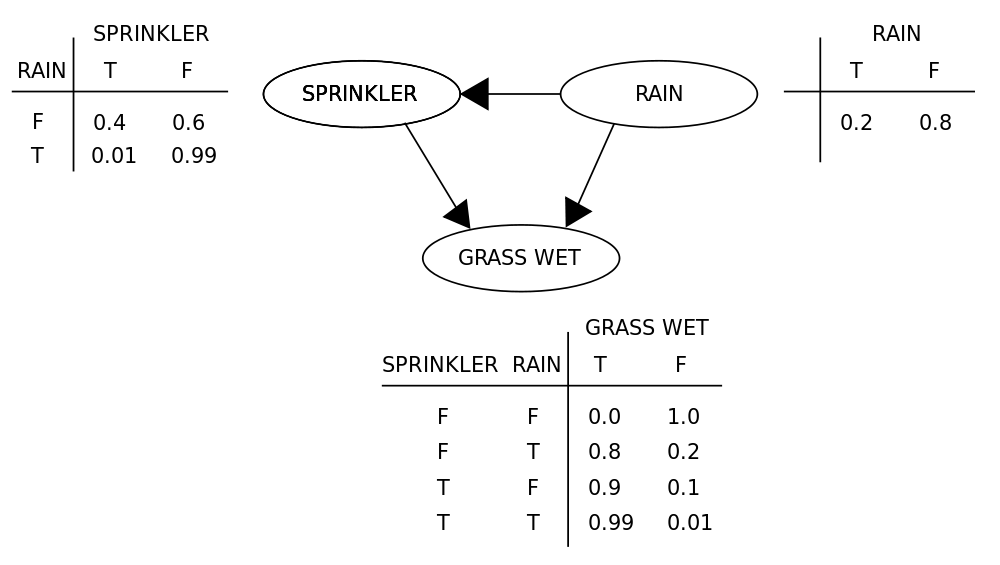
\includegraphics[width=\textwidth]{img/bayesian_example.png}
\caption{An example of a very simple bayesian network} \label{fig:bayesian_example}
\end{figure}

In our case, the nodes in the graph would represent all the different types of alarms which can be risen by our system. These nodes would have two possible states each: \emph{yes} (or \emph{true}) and \emph{no} (or \emph{false}) in a boolean fashion, indicating whether the alarm is risen or not within the observed period. Nodes in the graph are connected to each other through edges, which represent the causal influential relationship existing between them. Each state in a node (\emph{yes} or \emph{no}) is given a percentual value, indicating the probability of that state to be true or false in our system. These values are calculated as a function of their related nodes by application of Bayes theorem. This way, the probability of the \emph{yes} state of a node will be given by the probabilities of their parent nodes, each of which can affect it in a different way depending on the \emph{weight} of the edge connecting them.

\subsection{Construction of bayesian networks}
The creation of a Bayesian Network involves two different steps. First of all, we must obtain the graph structure for the network. This can be be achieved through different processes. The most convenient is to count on an already existing causal information for the nodes in our system. For example, if some of our nodes represent diagnosis systems results, and some other nodes represent possible errors, we may count already on information on which diagnosis systems can detect each of the errors and manually create a structure in that specific way. However, there might be scenarios in which these relations are completely unknown or not evident at first sight. In that case, we can also build these structures based on already existing data about the nodes in our network. In our case, we initially do not count on already existing relational information for our system, so the second approach will be followed. This way, we will create a preliminary structure with several relations between nodes. Using this information, we will check with Thales' engineers how each edge relates with actual causal relations (for example, systems which are known to be dependent of each other) and which ones are known to be completely unrelated (for example, independent systems which cannot have any influence in each other at all). Using this information we will \emph{tune} the preliminary structures manually strengthening those edges known to be valid and weakening or eliminating those known to be invalid.

The second step is to calculate the probability functions for all the nodes in the network. Once we have created the structure of our network --either manually or with automatic procedures-- we have to give states in each node a probability function, or in other words, calculate the weights of the edges. This process requires of large amounts of data to be used as evidence, from which the probabilistic dependencies will be calculated.

There are lots of available tools which already implement methods for these purposes. Specifically, we will use \emph{GeNIe/SMILE}\cite{druzdzel1999smile} as well as \emph{R libraries} in order to achieve this.

\subsection{Using bayesian networks to predict events}
%TO DO
\subsection{Validation and Evaluation}
% TO DO
\section{Model comparison: Bayesian Networks and Association rules}

At this point we have developed two predictive tools. First of all, we have obtained different sets of associative rules which we can use to make predictions based on and for different time windows. These rules must be now implemented into a Rules/Event processing platform such as JBoss Drools, which would take past events as an input and generate predictions based on the rules we have previously obtained.

Furthermore, we have developed an alternative tool following a different approach: \emph{Bayesian networks}. These networks are a mathematical tool which offer a causal model indicating how all the nodes in our network affect each others in terms of probability. In our bayesian networks, our nodes are all the possible alarms which can happen in our observation periods, which are related by their conditioned probabilities. When an event happens in our observation period, we can set the probability on that node to 100\% (we certainly know it has happened) and all the probabilities for other nodes will be recalculated according to the conditioned probabilities formulas in each of the edges of the graph.

\emph{Bayesian networks} are themselves a form of information in the form of a graph. The conditioned probabilities relating the nodes can sometimes show relations with actual implied causality in them. These relations are, however, generally not evident or not even real, as the high complexity of the network can propagate conditioned probabilities through non-related nodes, which - although matematically correct - would not represent actual causal relations.

For our purposes, both tools would be used in a similar fashion: we receive an input (the alarms which have happened during the current period) and want to generate a list with possible events and their probability. Whether the prediction is given by firing a set of rules or calculating probabilities with a bayesian network is of few importance to us. We will therefore analyse both models and choose the one which offers the best performance.

\subsection{Accuracy vs antecedent support}
The most important performance measure we will check is probably the accuracy or precision which can be achieved by both systems. We must however be careful when comparing both models, as predictions are not \emph{raised} with the same procedure in both of them. Specifically, we will also check the amount of alarms we need to know beforehand in order to give a valid prediction - given a precission threshold above of which we will consider our predictions good enough.

To begin with, we will check the maximum achievable precision with both system, for each number of antecedents considered. In the case of association rules this means the number of alarms needed for the rule to be risen, and in the case of bayesian networks, the amount of nodes we must set to 100\% probability (i.e. already happened) to obtain those values. It is important to note that in the case of association rules, we have set the cSPADE algorithm to search sequences in depths of a maximum of 7 events, as higher sequences could otherwise not be handled by our available systems.

The results can be seen in table \ref{tab:accuracy_cspade_bn} and figure \ref{fig:accuracy_cspade_bn}.

\begin{table}
\begin{center}

\begin{tabular}{|c|c|c|}
\hline \headcell{$ max\{size_{ant.}\}$} & \headcell{$ max\{prec_{rules}\}$} & \headcell{$ max\{prec_{BN}\}$} \\ 
\hline
\hline 1 & 0.43 & 0.01 \\ 
\hline 2 & 0.51 & 0.01 \\ 
\hline 3 & 0.83 & 0.02 \\ 
\hline 4 & 0.83 & 0.02 \\ 
\hline 5 & 0.83 & 0.03 \\ 
\hline 6 & 0.83 & 0.03 \\ 
\hline 7 & 0.83 & 0.04 \\ 
\hline 8 & -- & 0.06 \\ 
\hline 9 & -- & 0.09 \\ 
\hline 10 & -- & 0.15 \\ 
\hline 11 & -- & 0.18 \\ 
\hline 12 & -- & 0.18 \\ 
\hline ... & ... & ... \\ 
\hline 20 & -- & 0.24 \\ 
\hline 21 & -- & 0.24 \\ 
\hline 22 & -- & 0.24 \\ 
\hline 

\end{tabular} 
\caption{Maximum precision for association rules and bayesian networks} \label{tab:accuracy_cspade_bn}
\end{center}
\end{table}


\begin{figure}[hbtp]
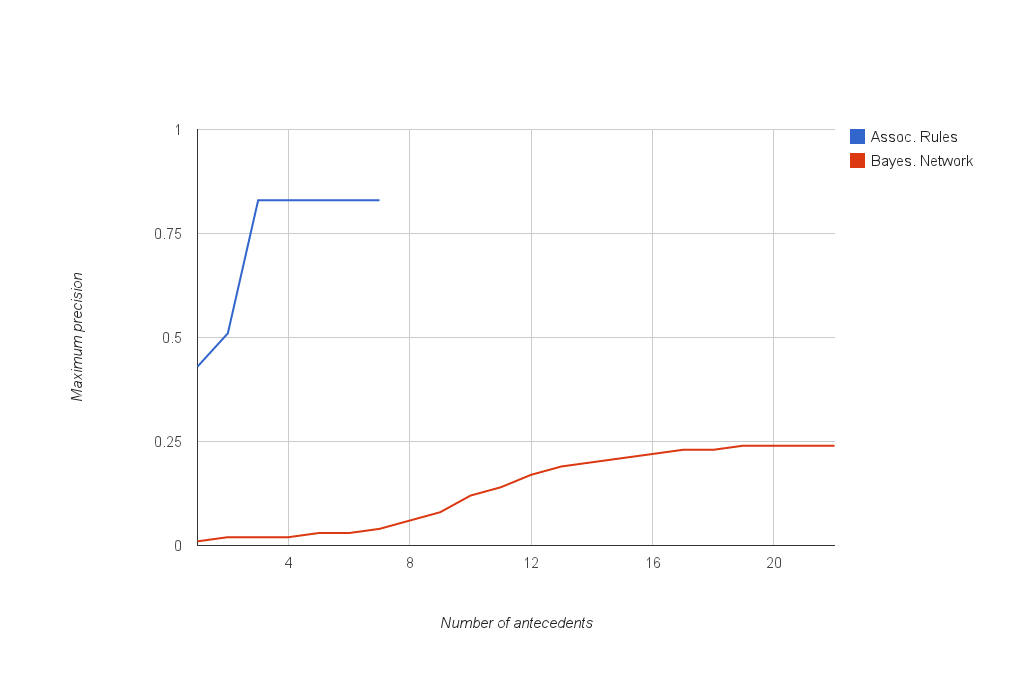
\includegraphics[width=\textwidth]{img/assoc_vs_bayes.png}
\caption{Maximum precision for association rules and bayesian networks} \label{fig:accuracy_cspade_bn}
\end{figure}

In figure \ref{fig:accuracy_cspade_bn} we can see at first glance that Bayesian Networks perform poorly in terms of accuracy. Whilst they give information on probability for all the possible events in our system, they cannot achieve such high precissions as our rule-based model. It is important to note that we have not considered number of antecedents higher than 22, because that is the standard value of different alarms raised over periods of days. This value does not vary significantly over periods of weeks, and we would have to study periods of months or years to probably get better results. As we do not count on such long periods (we would need to count on several years to make predictions in terms of years), this option cannot be evaluated.

On the other hand, we find that the maximum precision for rule-based predictions is achieved already in rules with three terms in the antecedent. This results in much more convenient knowledge, as having to wait till we receive a high number of different alarms in order to be able to predict anything is indeed a poor performing method.

In order to avoid these results to be unrealistic due to maximum-performance values which could be outliers, we will make a deeper insight on the number of predictions we would be able to make in each case. In the case of association rules, this is the number of rules whose precision is higher than our defined threshold, and in bayesian networks, the number of nodes of which we can make a different prediction with a higher precision. In this case, we will not limit the maximum number of alarms to be taken into account.

As the number of rule sets and bayesian networks which we can build is very high, we will illustrate this with an example case taking the \emph{Antequera} maintenance station.

\begin{table}
\begin{center}

\begin{tabular}{|c|c|c|}
\hline \headcell{$ min\{prec\}$} & \headcell{$ num\{pred_{rules}\}$} & \headcell{$ num\{pred_{BN}\}$} \\ 
\hline
\hline 0.80 & 48 & 0 \\ 
\hline 0.70 & 787 & 0 \\ 
\hline 0.60 & 2872 & 0 \\ 
\hline 0.50 & 3795 & 0 \\ 
\hline 0.40 & 6095 & 0 \\ 
\hline 0.20 & 14340 & 100 \\ 
\hline 0.10 & 18727 & 350 \\ 
\hline 0.05 & 22308 & 560 \\ 
\hline 

\end{tabular} 
\caption{Number of possible predictions for each precision value} \label{tab:numrules_cspade_bn}
\end{center}
\end{table}

In table \ref{tab:numrules_cspade_bn} we can clearly see that our rule-based model performs much better in general terms. Higher precision values of 0.83 were not caused by outliers, but there is an exponential progression in the number of predictions we can make with each precision threshold. It is important to note that these values depend on the exact model we are comparing (we will have --at least-- one per maintenance station), however, in general terms association rules perform much better than bayesian networks.

\subsection{Predictive information handling}
One of the issues we want to have into account is how to handle and maintain the knowledge we have acquired for future usage. In this direction, we have a huge difference between both tools: association rules are completely independent from each other, while the bayesian network can only function as a whole and complete system. In this direction, association rules offer a much higher flexibility for any kind of task we would like to perform in the future. Whether we would like to only monitor a specific type of event, or modify some variables in our prediction module according to changes in our systems, association rules offer a high advantage here over bayesian networks, as whichever of these tasks would be easily performed by someone without any data-mining knowledge in the first case, and would require of advanced training on bayesian models in the second.

\subsection{Model choice}
Given these performance comparisions, it is clear that we can achieve much better results using association rules than using bayesian networks. Bayesian networks can be much further tuned and trained in order to achieve much better performance, a task which requires understanding of the events nature and relations, as well as a deep analysis and evaluation of different sub models.

There are also other performance measures that can be taken into account, such as execution times for the prediction engine or computational cost of the model acquisition. However, these measures are by far not as important as the one we have taken into account here: prediction accuracy, in which bayesian networks have so far performed much worse than our rule-based model. 

For these reasons, our work has been focused on the rule-based model, which has already proven since earlier comparisions a much better performance.

\section{Result details and evaluation}


\clearpage

\bibliographystyle{plain} 
\bibliography{datamining}

\end{document}


